% вторая часть

\section{Разработка архитектуры микродрона}
\subsection{Аппаратная часть}

Набор наземной станции и квадрокоптера в основном планируется использовать в помещении. В случае использования БПЛА на улице, при весе свыше 250г требуется регистрация, согласно воздушному кодексу Российской Федерации\cite{ivp} . Основываясь на этом, поставлены следующие условия к компонентам квадрокоптера:

--- размер не должен превышать 140*140*50 \(мм^3\),

--- полетный вес должен быть ниже 250 г,

--- квадрокоптер должен выдерживать столкновения,

--- пропеллеры должны быть защищены,

--- минимальное полетное время 5 мин,

--- энергопотребление?

Подходя к вопросу выбора рамы, стоит учитывать такие факторы как:

--- прочность рамы,

--- легкий вес,

--- диагональную жесткость,

--- стоимость,

--- расстояния между отверстиями, совпадающие с монтажными отверстиями на электронике

Были проведены испытания с рамами из разных материалов. Рассматривались следующие альтернативы: фанера, PLA и PETG пластики, текстолит, углепластик (карбон). Фанера обладает низкой стоимостью, но уступает по жесткости остальным альтернативам. PLA пластик самый безопасный для здоровья человека, им можно печатать детали на 3d принтере, но не устойчив к ударам. PETG обладает большей прочностью по сравнению с ПЛА, но недостаточно жесткий, в связи с чем может вносить осцилляции в гироскоп, ухудшая работу ПИД регулятора полетного контроллера. Текстолит является самым жестким среди вышеперечисленных альтернатив, но обладает самым большим весом. Карбон уступает по стоимости, однако является самым прочным и относительно легким вариантом. Обладает достаточной жесткостью, благодаря чему не вносит нежелательные осцилляции. Таким образом, было решено ставить карбоновую раму.
Защита для пропеллеров пластиковая, так как обладает упругостью и низкой стоимостью.

Форм фактор рамы также является немаловажной деталью. Для выполнения задач, где используется направление камеры вниз, вперед и вверх необходимо, чтобы защита пропеллеров, пластины рамы, а также аккумулятор не загромождали обзор. Оптимальным решением является рама с вытянутым корпусом и расположением лучей по типу deadcat -- передние лучи разведены на угол, близкий к 180 градусам. Расстояние между отверстиями для монтажа электроники выгоднее выбирать из стандартов - 16*16, 20*20 или 25,5*25,5 мм. Вариант 25,5*25,5мм рассматривать стоит только в том случае, если необходимо использовать плату, где разведены и полетный контроллер, и регулятор. В этой работе такая плата неуместна, так как: в случае поломки заменяется полностью, стоимость больше, чем у регуляторов и полетного контроллера вместе, и выбор такой платы с ресурсами, необходимыми для реализации моего проекта, крайне мал. Основываясь на вышеперечисленном была приобретена рама, представленная на рисунке \ref{fig:frame}. Она позволяет установить нано камеру, стеки с монтажными отверстиями 20x20mm/16x16mm, моторы 1102-1308 и пропеллеры диаметром 40 мм.


\begin{figure}[H]
	\centering
	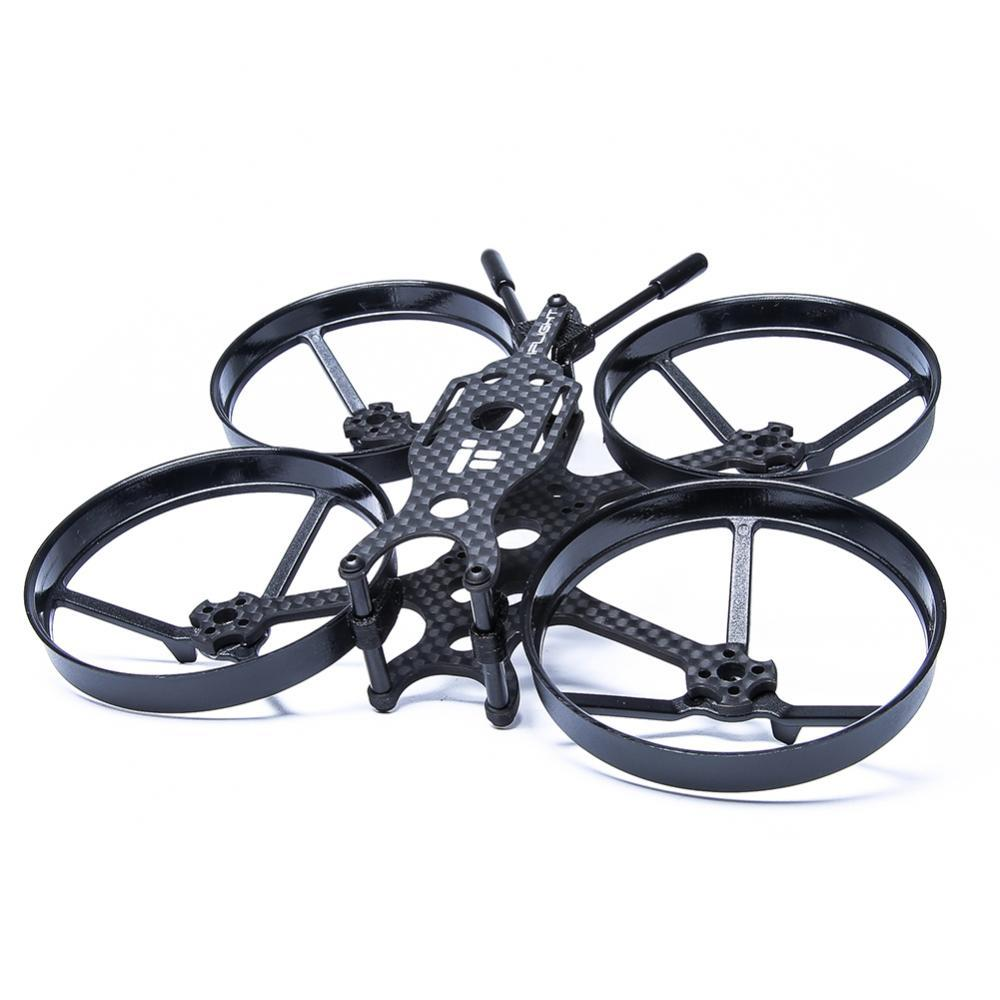
\includegraphics[width=0.5\linewidth]{pics/frame}
	\caption{Рама для экспериментального образца квадрокоптера
	}
	\label{fig:frame} % эта метка позволяет ссылаться на рисунок в тексте
\end{figure}

Электроника квадрокоптера должна быть совместимой по характеристикам и габаритам. Регуляторы оборотов существуют 2 типов: раздельные для каждого мотора и размещенные на одной плате с монтажными отверстиями, как у полетного контроллера. Для легкого БПЛА выгоднее ставить стек из платы с 4 регуляторами и полетного контроллера.
Для управления с наземной станции полетный контроллер должен:

--- обладать минимум 3 UARTами,

--- иметь процессор на базе F405/F745/F765 чипа

UART (Universal asynchronous receiver/transmitter) -- это аппаратный последовательный интерфейс, который позволяет подключать датчики и периферию к полетному контроллеру. У него есть два контакта: TX -- для передачи данных, RX -- для приема.

Выбор чипа процессора основан на количестве ресурсов. Для того, чтобы прошить PX4, необходим объем памяти процессора не ниже 1 МБ. Такое условие выполняют процессоры на базе F405/F745/F765.
% дописать
Винто-моторная группа должна быть оптимизирована под задачи автономного полета в помещении на небольшой скорости и вмещаться в выбранную раму. У бесколлекторных моторов основными параметрами являются размеры статора (4 цифры) и количество оборотов на вольт(kv). В четырех-значном числе первые два отвечают за диаметр статора, вторые -- за высоту статора. Чем больше диаметр статора, тем больше тяговооруженность мотора. Чем больше высота, тем больше скорость. Для экспериментально образца были выбраны трехлопастные пропеллеры с шагом 2.3 дюйма, диаметром 40 мм. Оптимальным выбором являются моторы 1202. Количество оборотов на вольт выберем, учитывая напряжение аккумулятора.
Для квадрокоптера с диагональю рамы 120 мм по соотношению вес / токоотдача наиболее выгодно ставить аккумуляторы с 2-3 ячейками. Каждая ячейка, подключенная последовательно увеличивает напряжение на 4.2 В в заряженном состоянии. Чем больше напряжение, тем меньше количество оборотов на вольт должно быть на моторе. Основываясь на таблице характеристик, приведенных производителем, были выбраны моторы с 6000 kv (рис. \ref{fig:motor}).
Учитывая потребление тока моторами на полном газу и добавляя 15 \% запаса, получаем характеристики регуляторов.
\begin{figure}[H]
	\centering
	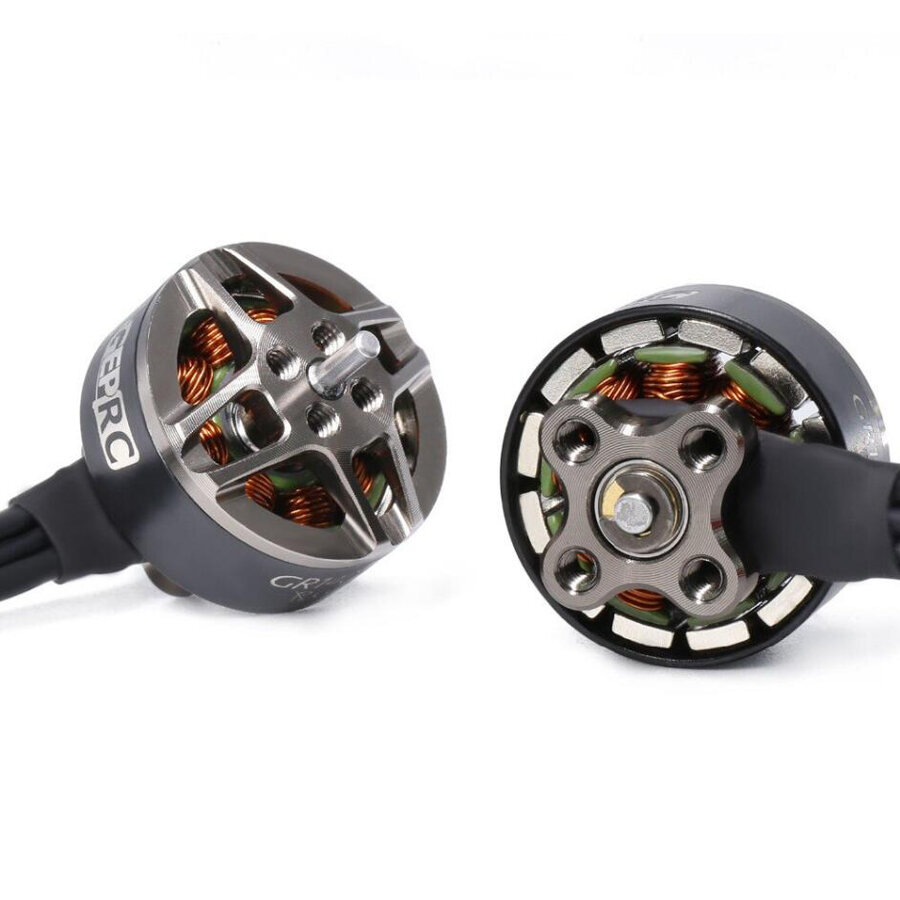
\includegraphics[width=0.5\linewidth]{pics/motor}
	\caption{Моторы для экспериментального образца квадрокоптера
	}
	\label{fig:motor} % эта метка позволяет ссылаться на рисунок в тексте
\end{figure}
\begin{figure}[H]
	\centering
	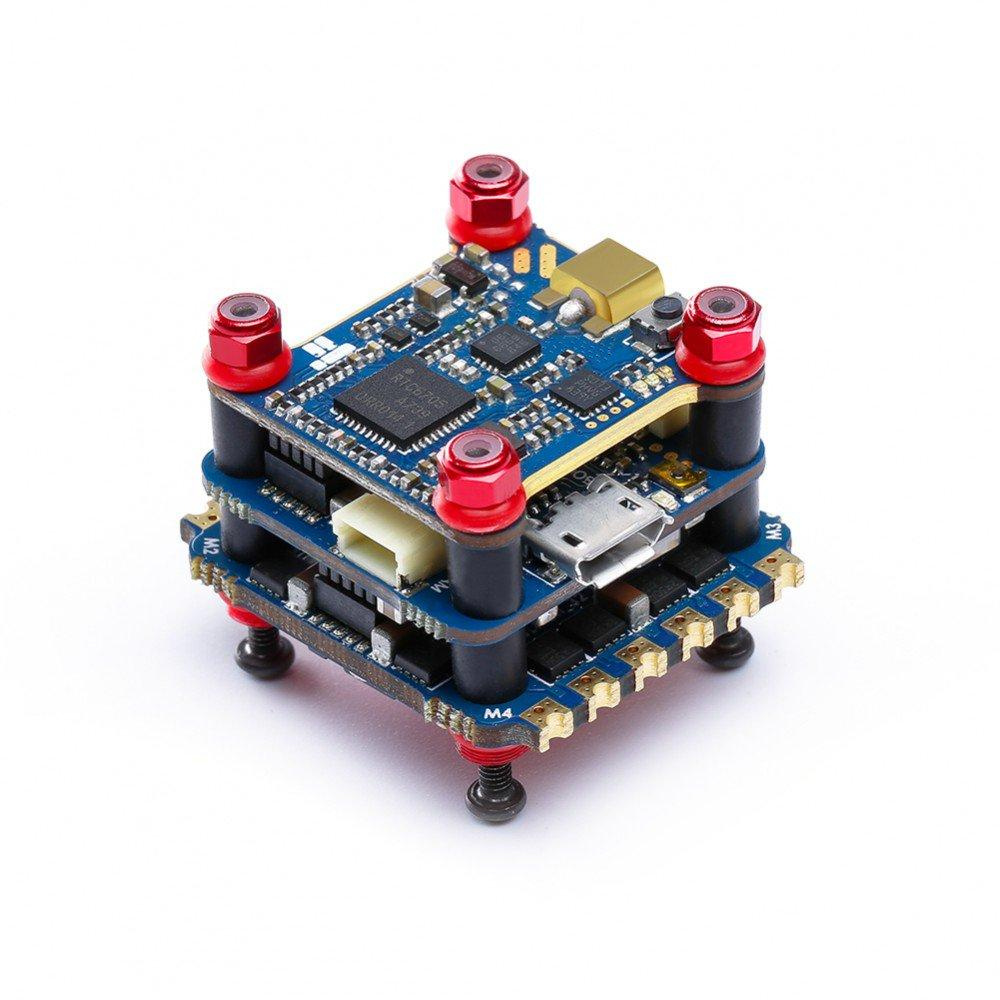
\includegraphics[width=0.5\linewidth]{pics/stack}
	\caption{Стек электроники для экспериментального образца квадрокоптера
	}
	\label{fig:stack} % эта метка позволяет ссылаться на рисунок в тексте
\end{figure}
Видеопередатчик и камера выбирались исходя из поставленных условий. Так как необходимо будет передавать видеопоток, камера должна иметь максимально возможное количество телевизионных линий (TVL). Для камер нано формата это 1000 TVL. Размер изображения может быть как 4:3 и 16:9. Формат PAL / NTSC также может быть выбран на усмотрение.

Видеопередатчик обладает такими характеристиками как:

--- выходная мощность,

--- частота передачи,

--- количество каналов

Для помещений мощность 25mW является оптимальной. Количество каналов должно быть выбрано таким образом, чтобы в случае совместных полетов сигнал не пересекался с чужим. Современные видеопередатчики имеют 40 каналов. Частота видеосигнала будет использоваться 5.8ГГЦ.

Для общения с наземной станцией понадобятся радиоприемник и телеметрийный модуль. Протокол и частота модулей станции и квадрокоптера должны совпадать.% дописать

\subsection{Программная часть}
В качестве прошивки для квадрокоптера был выбран PX4 - проект с открытым исходным кодом, позволяющий выполнять автономные полеты.
//почему был выбран рх4?
//его возможности?
//estimator (lpe)

\url{https://dev.px4.io/v1.9.0/en/ros/external_position_estimation.html}
